%%%%%%%%%%%%%%%%%%%%%%%%%%%%%%%%%%%%%%%%%
% Thin Sectioned Essay
% LaTeX Template
% Version 1.0 (3/8/13)
%
% This template has been downloaded from:
% http://www.LaTeXTemplates.com
%
% Original Author:
% Nicolas Diaz (nsdiaz@uc.cl) with extensive modifications by:
% Vel (vel@latextemplates.com)
%
% License:
% CC BY-NC-SA 3.0 (http://creativecommons.org/licenses/by-nc-sa/3.0/)
%
%%%%%%%%%%%%%%%%%%%%%%%%%%%%%%%%%%%%%%%%%

%----------------------------------------------------------------------------------------
%	PACKAGES AND OTHER DOCUMENT CONFIGURATIONS
%----------------------------------------------------------------------------------------

\documentclass[a4paper, 11pt]{article} % Font size (can be 10pt, 11pt or 12pt) and paper size (remove a4paper for US letter paper)

\usepackage[protrusion=true,expansion=true]{microtype} % Better typography
\usepackage{graphicx} % Required for including pictures
\usepackage{wrapfig} % Allows in-line images
\usepackage[paper=a4paper,left=25mm,right=25mm,top=25mm,bottom=25mm]{geometry}

\renewcommand{\familydefault}{\sfdefault}
\usepackage{helvet} % Use the Palatino font
\usepackage[T1]{fontenc} % Required for accented characters
\usepackage[format=plain,footnotesize,labelfont=bf,justification=justified,singlelinecheck=false]{caption}


\linespread{1.05} % Change line spacing here, Palatino benefits from a slight increase by default



\makeatletter
\renewcommand\@biblabel[1]{\textbf{#1.}} % Change the square brackets for each bibliography item from '[1]' to '1.'
\renewcommand{\@listI}{\itemsep=0pt} % Reduce the space between items in the itemize and enumerate environments and the bibliography

\renewcommand{\maketitle}{ % Customize the title - do not edit title and author name here, see the TITLE block below
\begin{flushright} % Right align
{\LARGE\@title} % Increase the font size of the title

\vspace{20pt} % Some vertical space between the title and author name

{\large\@author} % Author name
\\\@date % Date

\vspace{10pt} % Some vertical space between the author block and abstract
\end{flushright}
}

%----------------------------------------------------------------------------------------
%	TITLE
%----------------------------------------------------------------------------------------

\title{\textbf{Co-regulation of NER repair factor expression}\\ % Title
Third TAC-meeting} % Subtitle

\author{\textit{Tim Heinemann} % Author
\\{\textit{Theoretical Systems Biology (AG H�fer)}}} % Institution

\date{\textit{\today}} % Date

%----------------------------------------------------------------------------------------

\begin{document}

\maketitle % Print the title section

%----------------------------------------------------------------------------------------
%	ABSTRACT AND KEYWORDS
%----------------------------------------------------------------------------------------

%\renewcommand{\abstractname}{Summary} % Uncomment to change the name of the abstract to something else

%----------------------------------------------------------------------------------------
%	ESSAY BODY
%----------------------------------------------------------------------------------------

\section*{Introduction}

The recently published model-aided analysis of the DNA repair process revealed the link between the emergent phenomenon of rapidly exchanging and transiently interacting NER components with the experimentally observed slow first-order kinetics of repair \cite{Verbruggen2014}. An important functional consequence of this kinetic design is that the control of the repair rate is shared by all repair factors. This manifests in the mathematical prediction of uniformly distributed response coefficients, which quantify the relative change of the repair rate in answer to changes in the nuclear repair protein concentration. Exploiting the natural variability in NER factor expression we experimentally corroborated the moderate control of the repair components on the repair rate. However, these findings were made under the assumption of a functional independence of the individual NER components. Downstream  effects regulating the repair rate due to NER factor co-expression were so far not considered.  \\
To test this assumption, we experimentally investigate the potential cross-correlation between five repair factors (XPC, TFIIH, XPA, XPF and RPA). Surprisingly, we find that the nuclear expression of these pairwise measured repair factors is indeed strong positively correlated, whereas there is no correlation with the repair-independent cell cycle marker Ki67. This result suggests an additional control mechanism orchestrating NER factor expression on the transcriptional or translational level. 


\section*{Nuclear expression of NER factors is strongly correlated}

Using fluorescence microscopy for the quantitative analysis of the NER process proved to result in accurate measurements of the nuclear repair factor expression and their UV-induced repair dynamics at a high signal to noise ratio. This applies for the stably transfected fluorescently tagged repair protein expression as well as for an immunocytochemistry approach with an indirect antibody-labeling of the measured NER factors. Indirect labeling of the primary antibody with a secondary antibody allows for the combinatorial tagging of multiple antigens, which we established for seven single cell double stainings (XPC-XPC; XPC-TFIIH; XPC-XPA; XPC-XPF; XPC-RPA; TFIIH-XPF; XPA-XPF; XPA-RPA). 
The cross-correlation analysis was performed in	human diploid female fibroblasts. After the antibody labeling of two selected repair factors microscopic 3-dimensional imaging was conducted on a Leica TCS SP5 II confocal microscope.To test whether the antibody co-staining experiment is suitable for the cross-correlation analysis we measured XPC with a directly labeled antibody as well as an indirect labeling. We correlated both signals originating from the nucleus (cf.\ Figure \ref{fig:Mic_nucCorrel}A). the measurement error was determined with ..., Hence, this approach is sufficiently accurate to exploit the natural variability in protein expression for the cross-correlation analysis. 


\begin{figure}[htbp]
	\begin{center}
		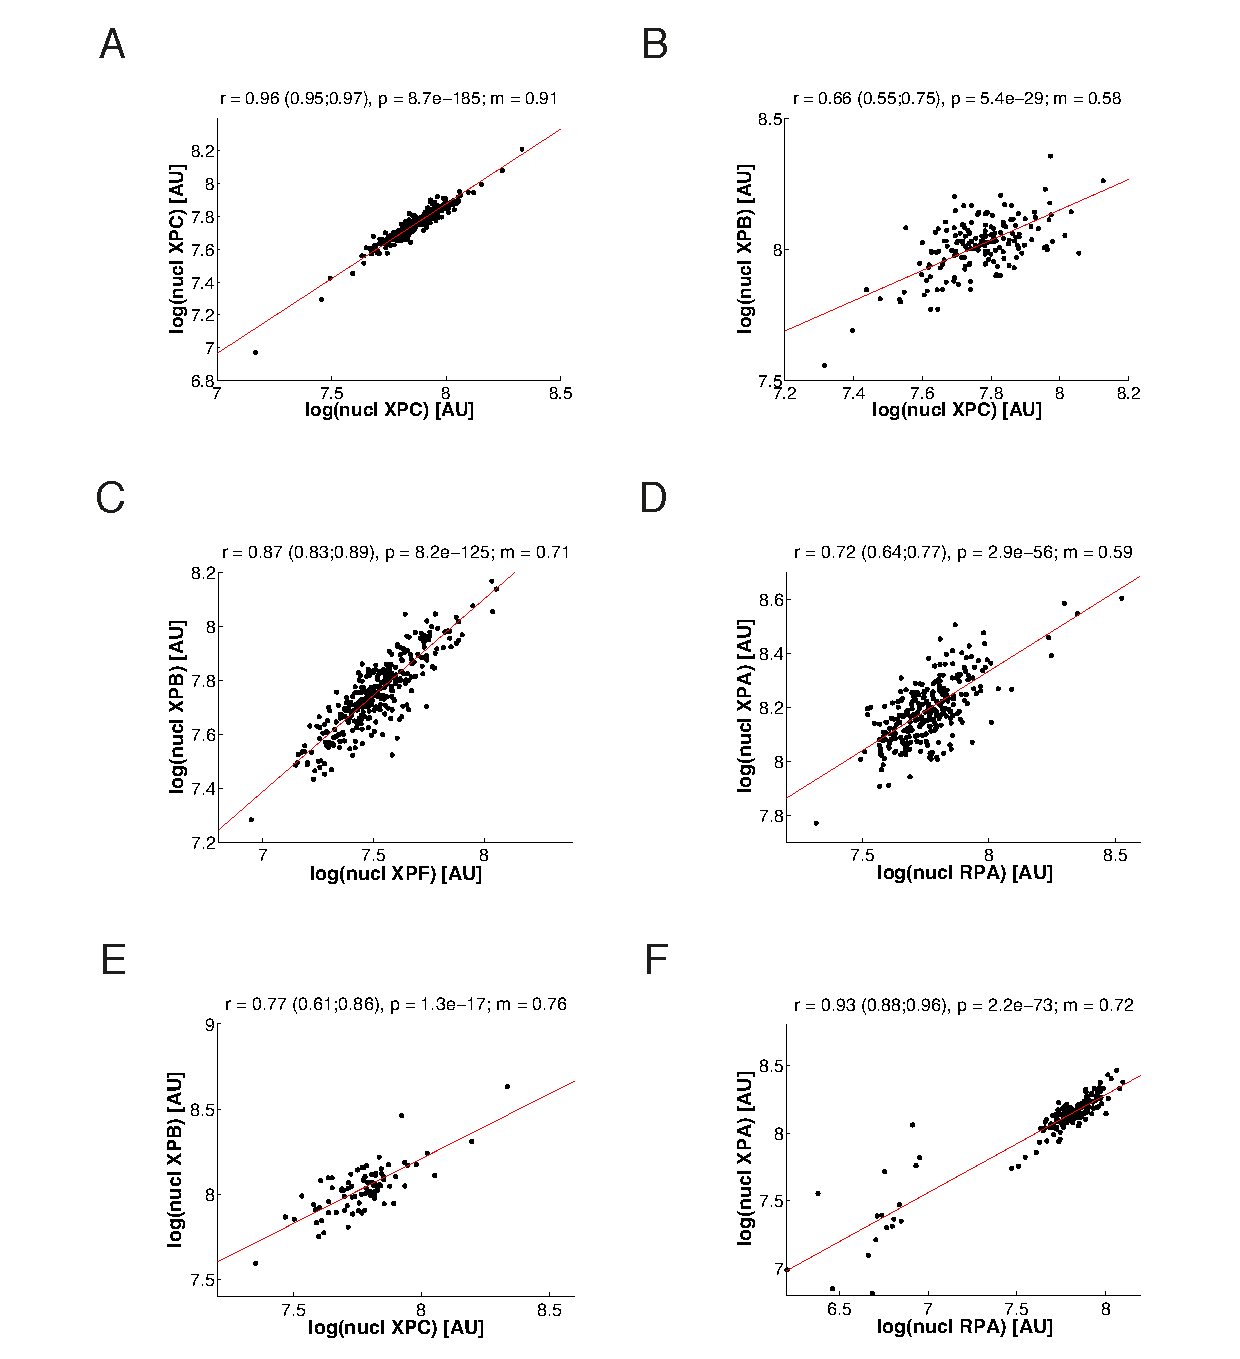
\includegraphics[width=1\textwidth]{Abbildungen/figureTAC_2.pdf}
		\caption{\textbf{Blubb.} A) B) }
		\label{fig:Mic_nucCorrel}
	\end{center}
\end{figure}


\noindent As it turns out, all pairwise correlations of the measured co-staining experiments are strong positively correlated with correlation coefficients between 0.74 and 0.88 (cf.\ Figure \ref{fig:Mic_nucCorrel}B-D (only selected pairs)). Notably, the result is indifferent whether the acquired fluorescence signal is taken from the whole cell nucleus including the locally damaged area or only from the undamaged chromatin region (cf.\ Figure \ref{fig:Mic_nucCorrel}B-D and \ref{fig:Mic_nucCorrel}E-F). This suggests that the correlation of nuclear NER factors is independent of the ongoing repair. As a consequence, we suspect the regulatory mechanism determining the protein concentrations on a preceding level like transcription or translation.  


\begin{figure}[htbp]
	\begin{center}
		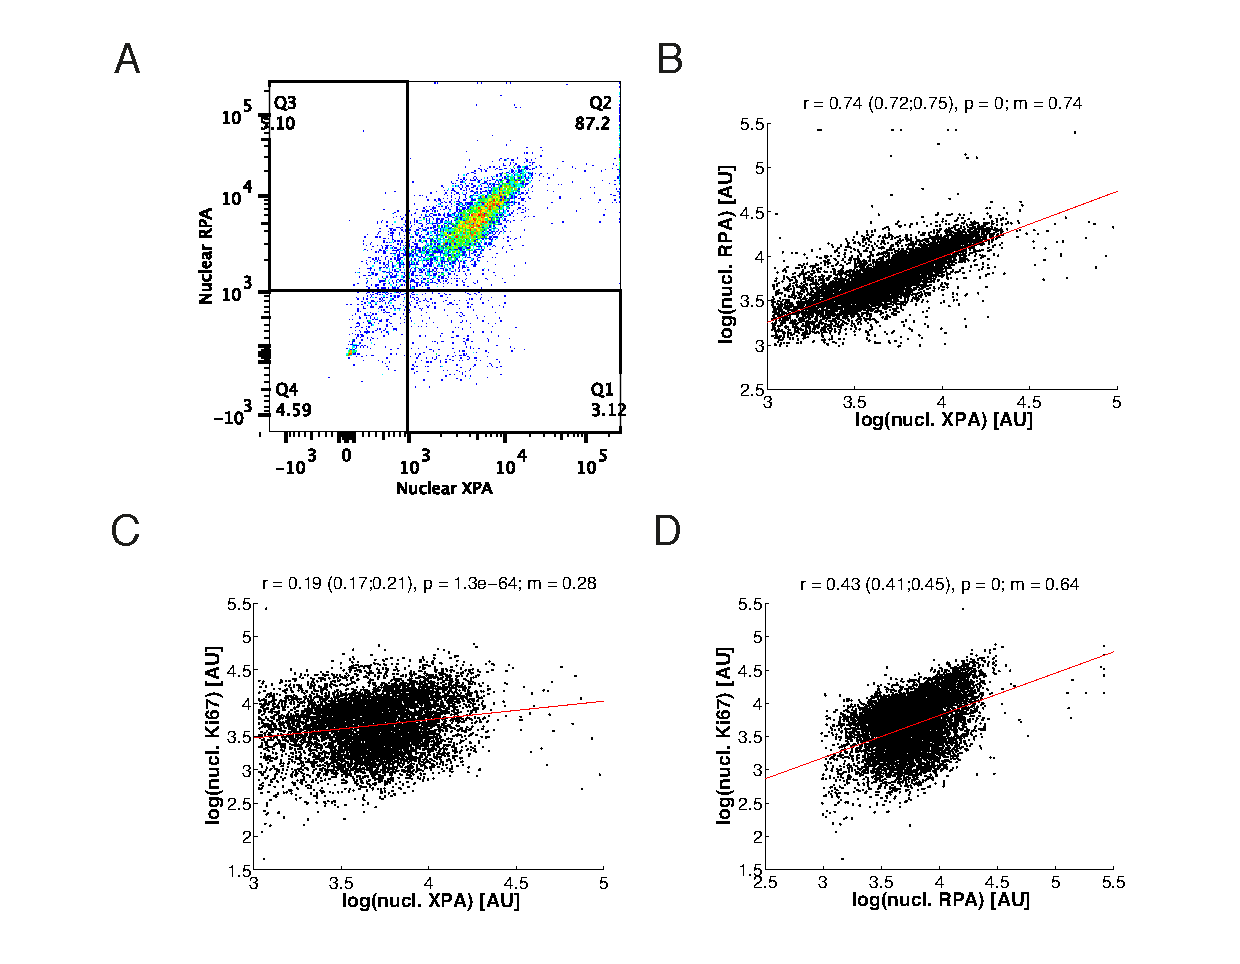
\includegraphics[width=1\textwidth]{Abbildungen/figureTAC_3.pdf}
		\caption{\textbf{Blubb.} A) B) }
		\label{fig:FACS_nucCorrel}
	\end{center}
\end{figure}

\section*{Cell cycle independent cross-correlation of NER factor expression}

%------------------------------------------------
\begin{figure}[htbp]
	\begin{center}
		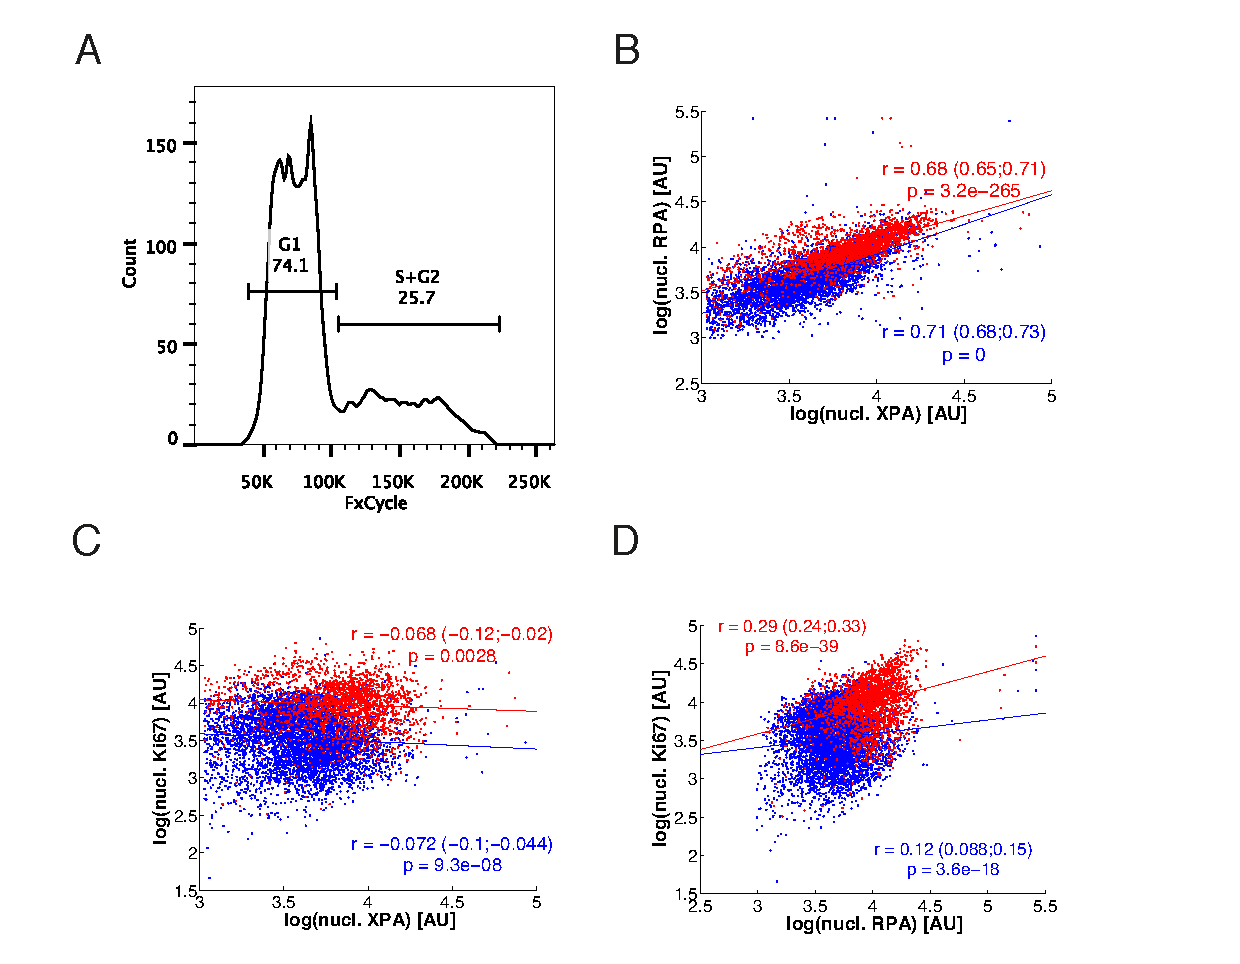
\includegraphics[width=1\textwidth]{Abbildungen/figureTAC_4.pdf}
		\caption{\textbf{Blubb.} A) B) }
		\label{fig:CellCycle_nucCorrel}
	\end{center}
\end{figure}



\section*{Conclusion}

The positive pairwise correlation of the nuclear repair factor concentration was conclusively shown by two independent experimental approaches. This implies that the abundance of a protein is dependent on the other repair components, which has to be considered when determining the control on the rate of repair.



%----------------------------------------------------------------------------------------
%	BIBLIOGRAPHY
%----------------------------------------------------------------------------------------

\footnotesize\bibliographystyle{naturemagC}
\bibliography{NER_Bibliography}

%----------------------------------------------------------------------------------------

\end{document}